\section{Shashlik + Hadron Endcap} \label{section:simulations_shashlik}
\begin{figure}[htbp]
    \centering
    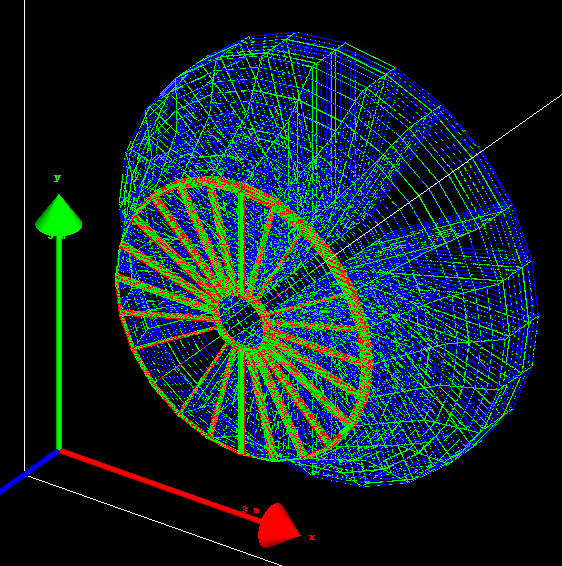
\includegraphics[width=0.9\textwidth]{figures/ch_simulations/shashlik/geometry/Shashlik+HE_Complete_Wire.png}\\
    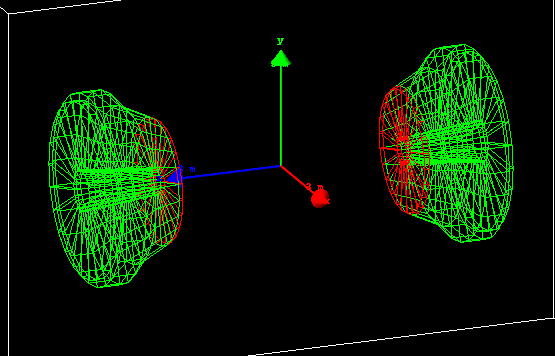
\includegraphics[width=0.9\textwidth]{figures/ch_simulations/shashlik/geometry/SHE_70_20.png}
    \caption{Full CMS Scale Shashlik + HE System (from different angles)}
    \label{fig:higgs_simulations_shashlikexamples}
 \end{figure}

\subsection{Physical Layout}
Shashlik is an Electromagnetic Calorimeter System with the name implicitly reflecting its structure and the choice of readout technology. The physical layout is similar to HGC~\ref{section:simulations_hgc}: alternating layers of absorber and active materials, however there is no electronics unit sitting on the calorimeter itself. Instead, wave-length shifting fibers go through the whole length of the calorimeter and are responsible for light capture and transmission to the electroncs unit for conversion into analog signal. Full specification of the Shashlik Calorimeter can be summarized as follows:
\begin{itemize}
    \item 25-30 $X_0$ device
    \item No Longitudinal Segmentation
    \item Alternating layers of absorber (tungsten W) and active (LYSO) materials.
    \item Active Material used is LYSO plastic scintillator.
\end{itemize}
Hadron Endcap (HE) is an active CMS Endcap Calorimeter that is part of the HCAL subsystem. Design principles are similar with respect to Shashlik, however has a slightly different choice of readout technology \cite{Baiatian:2008zz}. Calorimeter specification can be summarized as follows:
\begin{itemize}
    \item $10\lambda$ device
    \item Alternating layers of absorber (Brass) and active (SCSN-81 plastic scintillator) materials
    \item Partial Longitudinal segmentation.
\end{itemize}

\subsection{Detector Readout}
For the purpose of simplification, in the simulation the assumption is made to have a perfect light capture and transmission for both Shashlik and Endcap. Also no modeling of the wave-length shifting fibers or any kind of photodetectors. In other words, looking for upper limits of our calorimeter performance. The metric of the system's response is defined to be the number of generated photons within the scintillator. Scintillation mechanics is responsible for light generation and \textbf{G4Scintillation}, \cite{geant4}, physics process of {\sc Geant4} provides these capabilities via \textbf{optical photons}. For the purpose of modeling, {\sc Geant4} defines two different types of photons: regular photons, that obey the laws of quantum physics, and optical photons, that follow the laws of geometrical optics. Optical photons do not participate in the conservation of energy laws and do not deposit any energy into the scintillator (this fact allows for optimizations).

\subsection{Parametrized Detector Readout}
Typical light yields for a scintillator are in thoughsands of optical photons per MeV of deposited energy into the scintillation material. The exact number is material-dependent and varies substantially. Given that the input particle has energies in the GeV range, the number of optical photons that gets generated goes well above 1 M. Tracing all of these photons is a complicated and time-consuming task for Geant's engine. Moreover, given that \textbf{optical photons} can not deposit energy into the material, one can simply \textbf{count and kill} them right after they've been generated. Therefore, for the purpose of optimizing the time it takes to generate a single event, the parametrization of the response of a schintillator is performed. This procedure allows to substantially speed up the simulation without degrading the performance.

\subsection{Analysis and Results}
The analysis procedure is identical to the one described for HGC in section~\ref{section:simulations_hgc} and will not be repeat here. There are 2 main differences: first, the readout metric here is defined to be simply the total number of generated optical photons. No weighting layer by layer applied for neither Shashlik nor HE. And second, HE is calibrated separately, by shooting pions with a different set of energies. Figure \ref{fig:simulations_shashlik_linearity} shows the results of computing the linearity for both Shashlik and HE. It is clear, especially comparing to {\sc HGC}, that Shashlik exhibits better linearity properties.
 \begin{figure}[htbp]
    \centering
    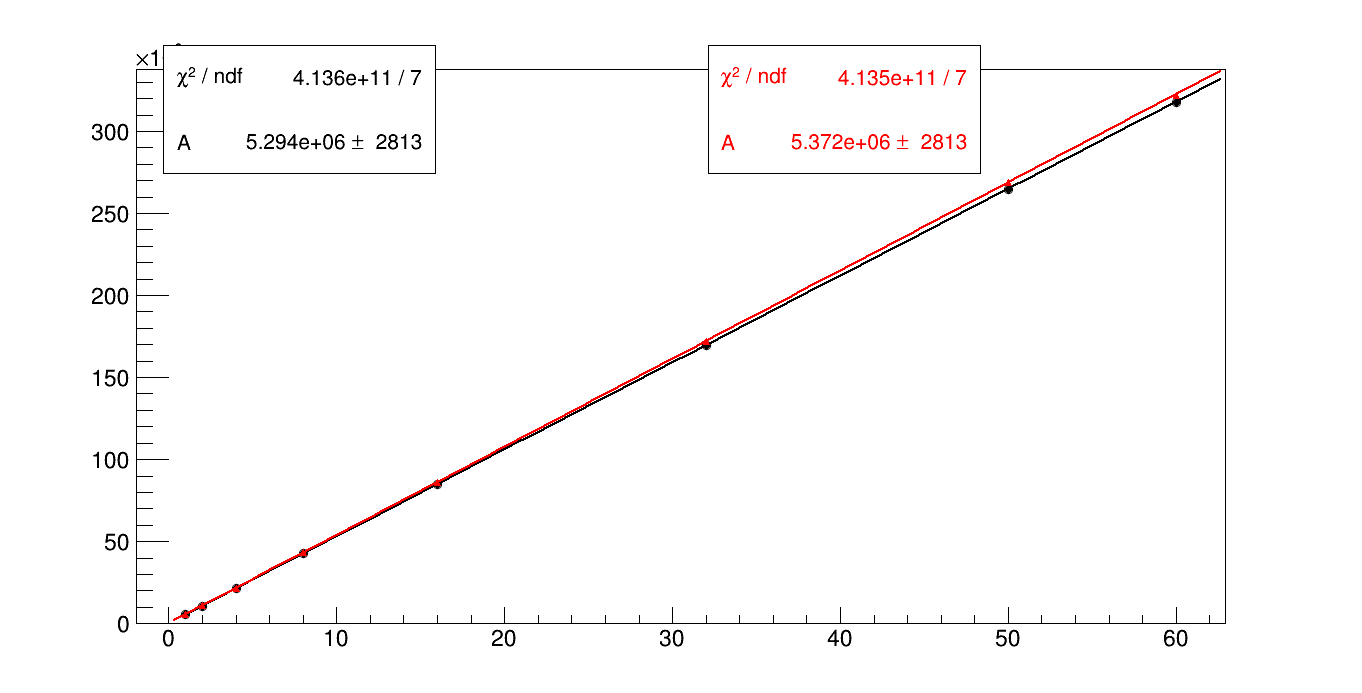
\includegraphics[width=0.95\textwidth]{figures/ch_simulations/shashlik/performance/ResponseVsEnergy.png}\\
    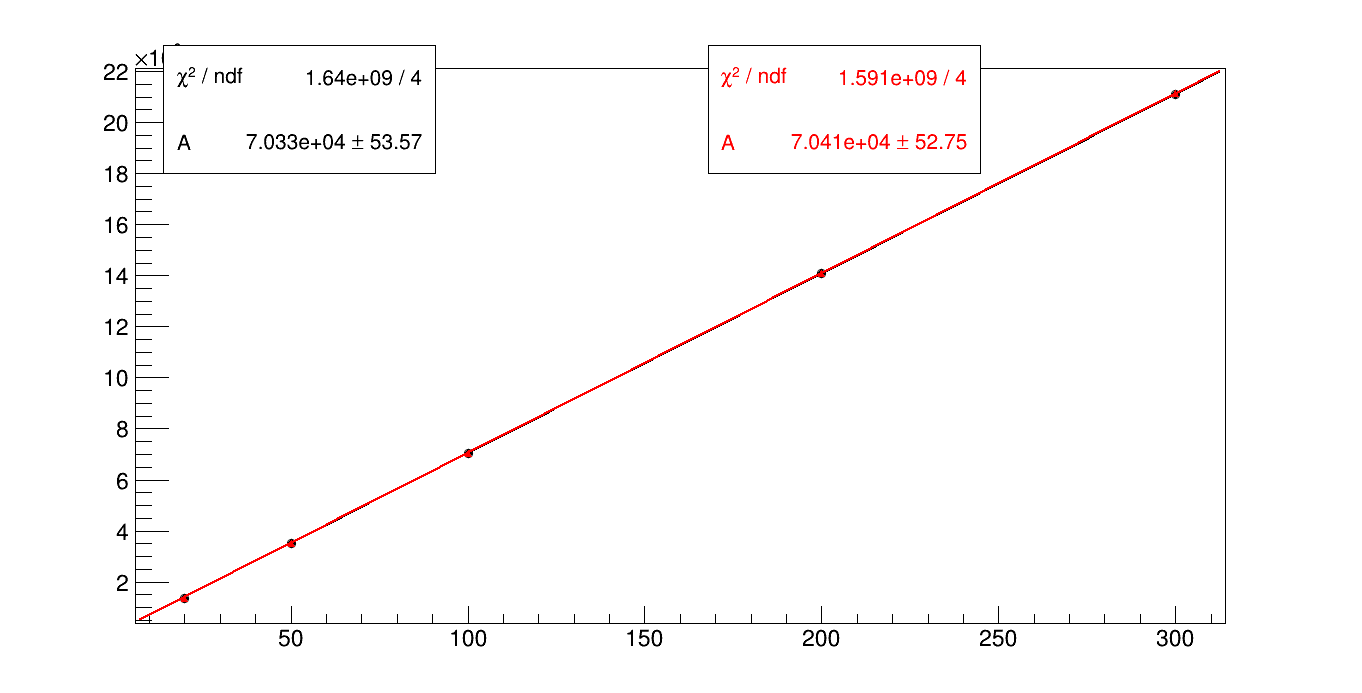
\includegraphics[width=0.95\textwidth]{figures/ch_simulations/he/performance/Linearity.png}
    \caption{Shashlik's Linearity (Top) and Hadron Endcap Linearity (Bottom)}
    \label{fig:simulations_shashlik_linearity}
 \end{figure}

Figures \ref{fig:simulations_shashlik_energyreco}, \ref{fig:simulations_he_energyreco} shows the reconstructed energy distributions for Shashlik and HE, respectively. Shashlik and HE are calibrated separately as they constitute isolated parts of the system. Note this is different with repsect to HGC, where calibration of EM and FH parts was done together.
\begin{figure}[hbtp]
    \centering
    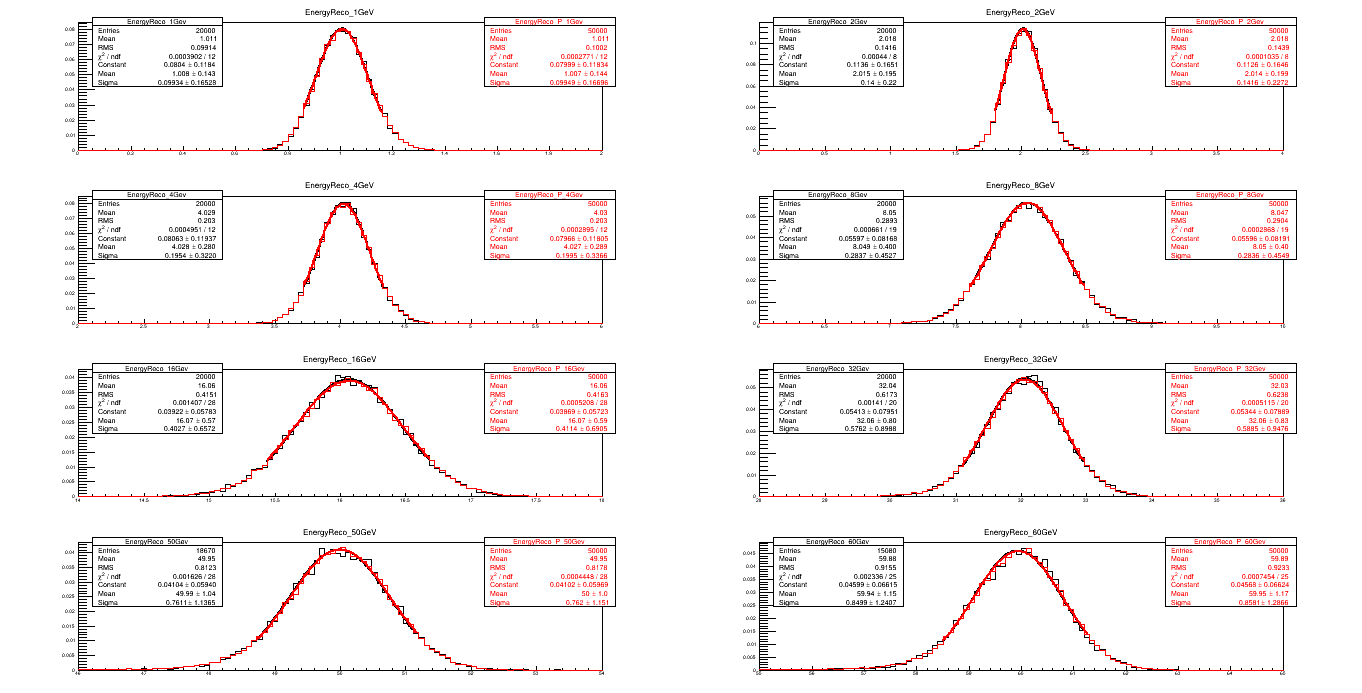
\includegraphics[width=0.95\textwidth]{figures/ch_simulations/shashlik/performance/EnergyRecoDistributions.png}
    \caption{Reconstructed Energy Distributions for Shashlik}
    \label{fig:simulations_shashlik_energyreco}
 \end{figure}
 \begin{figure}[hbtp]
    \centering
    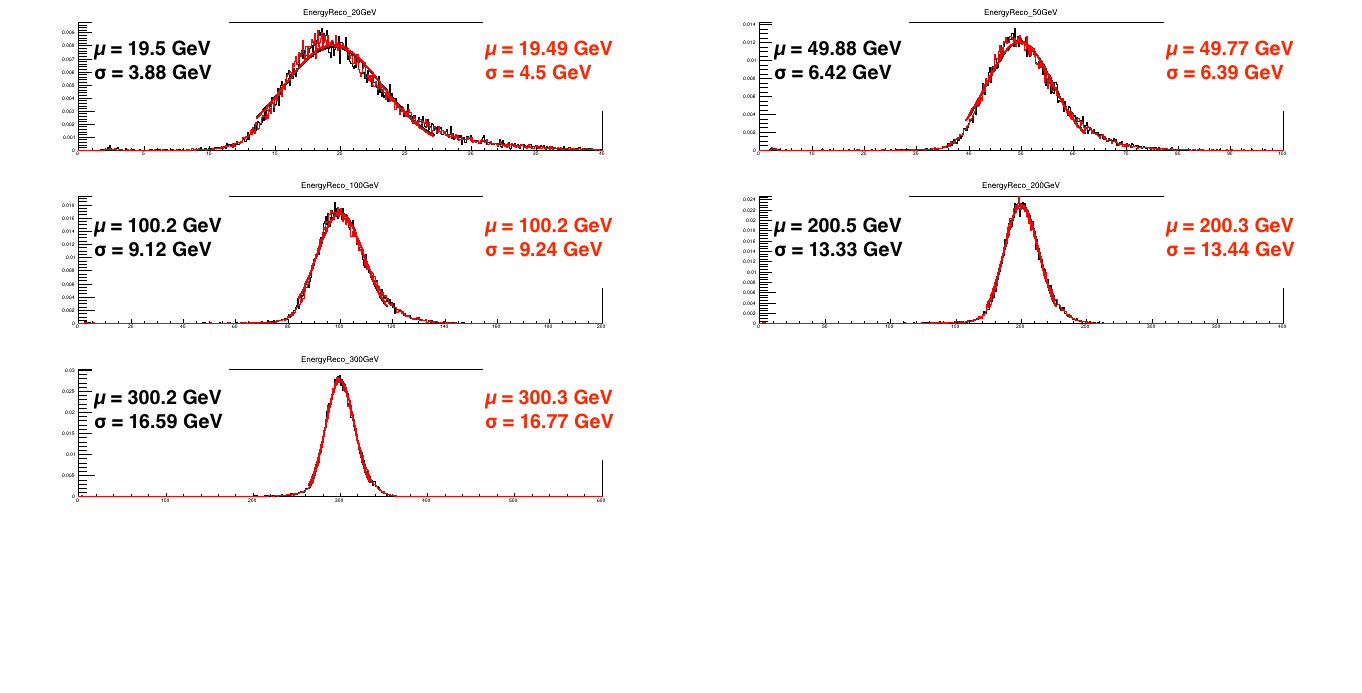
\includegraphics[width=0.95\textwidth]{figures/ch_simulations/he/performance/EnergyRECODistributions.png}
    \caption{Reconstructed Energy Distributions for Hadron Endcap}
    \label{fig:simulations_he_energyreco}
 \end{figure}

 Results for the energy resolution are provided in figures \ref{fig:simulations_shashlikhe_resolution}. The differences between the parametrized response and the use of optical photons is negligible.
 \begin{figure}[htbp]
    \centering
    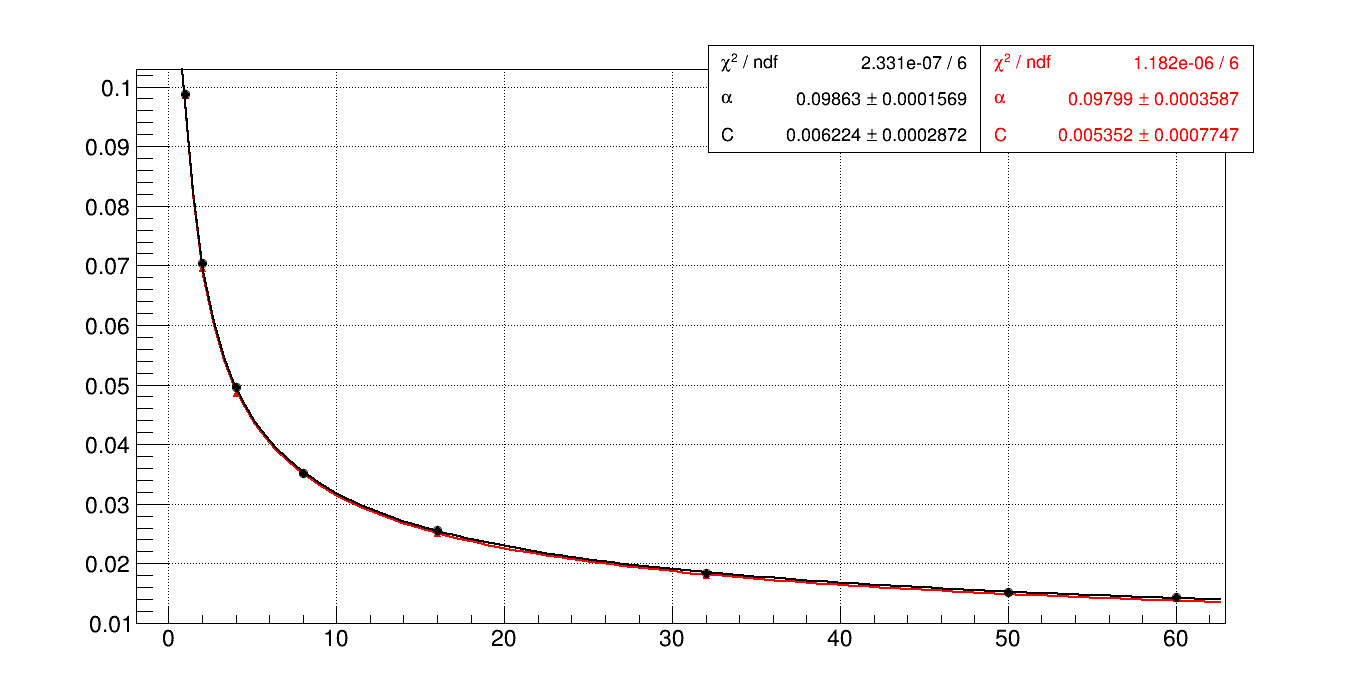
\includegraphics[width=0.95\textwidth]{figures/ch_simulations/shashlik/performance/energyResolution.png}\\
    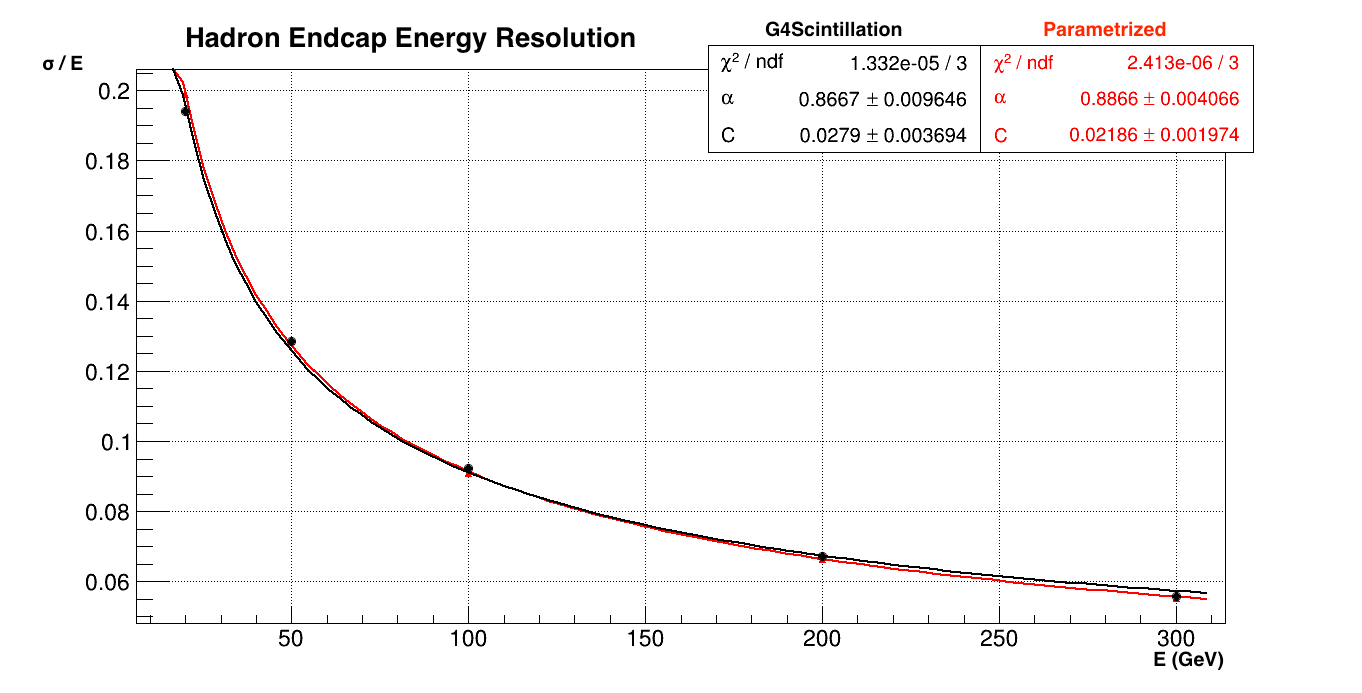
\includegraphics[width=0.95\textwidth]{figures/ch_simulations/he/performance/Resolution.png}
    \caption{Energy Resolution Shashlik (Top) and Hadron Endcap (Bottom)}
    \label{fig:simulations_shashlikhe_resolution}
 \end{figure}